\chapter{Authentication and identity management}
\label{chap:autenticazione}

\section{Request lifecycle}
\label{sec:ciclo-richiesta}

A registration or login request passes through three services before becoming a record:
Entry-Hub, Security-Switch, and Database-Vault. All three apply the same checks to the input,
each one independently of the others.

Validation takes place in two phases. The first concerns the request body: the payload is
read up to a limit of 2048 bytes and rejected if it exceeds it, and the JSON decoder rejects any unexpected field.

The second phase concerns the individual fields \cite{ramusb-code-eh-f-04}. The email must be a
single, syntactically valid address according to RFC 5322 \cite{rfc5322}; the password must be
between 8 and 128 characters long and use at least three categories among lowercase letters, uppercase letters, digits, and symbols.
At registration, moreover, the SSH public key must be well formed.

If a check fails, the response is HTTP 400 without indicating which check did not pass, the
log records the problem without identifying the user, and the request does not proceed inward.
The message stays generic because a detailed error would help an attacker more than it helps a
user acting in good faith, whose own client has already applied the same checks.

The three services share the same validation library, so repeating the check does not
introduce algorithmic diversity, but it guarantees that no service takes for granted that the
previous one did its job. In this way, if, for example, a tampered request coming from a
compromised service were to reach Database-Vault, the validation would still be performed and would cause the request to be discarded.

Finally, internal errors are translated into HTTP status codes. \autoref{tab:codici-http} summarizes the codes
that reach the user, attributing each code to the service that emits it.

Entry-Hub builds only the errors that originate in itself: a failed validation and a
call to Security-Switch that went wrong. Everything else it relays back to the client exactly as it arrives
from the inside, without modifying it. For this reason, a 401 or a 409 reaches the user despite never
being produced by Entry-Hub.

\begin{table}[H]
\centering
\caption{HTTP status codes returned to the client and their meaning in the system.}
\label{tab:codici-http}
\begin{tabular}{@{}l p{\dimexpr0.58\linewidth\relax} l@{}}
\hline
\textbf{Code} & \textbf{Meaning} & \textbf{Issued by} \\
\hline
400 & Validation failed, without indicating which check did not pass & both \\
401 & Invalid credentials, does not specify whether nonexistent email or wrong password & Security-Switch \\
403 & Explicit refusal from Network-Manager & Security-Switch \\
409 & Email or SSH key already registered, does not specify which of the two & Security-Switch \\
500 & Internal error not otherwise classified & both \\
502 & Downstream service unreachable or returning an unexpected response & both \\
503 & Call to Security-Switch timed out & Entry-Hub \\
504 & Call to Database-Vault or Network-Manager timed out & Security-Switch \\
\hline
\end{tabular}
\end{table}

The codes that the two services build on their own differ in two respects:
the first is 403, which only Security-Switch can emit, because it is the only one of the two that can receive an
explicit refusal from an internal service. The second concerns timed-out calls: Entry-Hub responds 503,
Security-Switch 504.

In all cases, the response body is sanitized and the error details remain in the internal
logs.

\section{Credential encryption and hashing}

Database-Vault treats the data it receives in three different ways:

\begin{itemize}
    \item the SSH key is public, so it does not require secrecy;
    \item the email is at the same time a lookup key and personal data to be protected, but it must also be
		recoverable when needed;
    \item the password must not be recoverable, not even by whoever administers the database.
\end{itemize}

The email is normalized to lowercase and reduced to its SHA-256 digest, which becomes the primary key
of the record. Normalization guarantees that the same address written with different letter case at login
produces the same key as at registration.
This hash is deterministic by necessity, because it must enable the lookup. The fundamental limitation of
this approach, together with its mitigation, is discussed in \autoref{chap:sicurezza}.

Alongside the digest that acts as the lookup key, the record keeps an encrypted copy of the email,
so that the address remains recoverable.
From a master key and a random 16-byte salt, generated for that record,
a dedicated key is derived with HKDF-SHA256 \cite{rfc5869}, with which the email is encrypted with
AES-256-GCM \cite{nist-sp-800-38d} using a random 12-byte nonce. Salt, nonce, and ciphertext
are stored in the record, while the derived key is zeroed as soon as the cipher has consumed it.
Deriving a key for each record, instead of encrypting everything with the master key, reduces the amount
of data protected by a single key.

\Needspace{22\baselineskip}
\begin{lstlisting}[caption={Per-record key derivation in \texttt{newGCM}, from
\texttt{encryption.go} \cite{ramusb-code-hkdf-newgcm}.}, label={lst:hkdf}]
func newGCM(masterKey, salt []byte) (cipher.AEAD, error) {
	derivedKey := make([]byte, derivedKeySize)
	kdf := hkdf.New(sha256.New, masterKey, salt, []byte(hkdfInfo))
	if _, err := io.ReadFull(kdf, derivedKey); err != nil {
		return nil, fmt.Errorf("encryption: derive key: %w", err)
	}

	block, err := aes.NewCipher(derivedKey)
	for i := range derivedKey {
		derivedKey[i] = 0
	}
	if err != nil {
		return nil, fmt.Errorf("encryption: new AES cipher: %w", err)
	}

	gcm, err := cipher.NewGCM(block)
	if err != nil {
		return nil, fmt.Errorf("encryption: new GCM: %w", err)
	}

	return gcm, nil
}
\end{lstlisting}


The password, instead, is concatenated with a pepper, read from an environment variable, and passed to Argon2id
\cite{rfc9106} together with a random 16-byte salt generated on the spot for that record.

OWASP \cite{owasp-password-storage} proposes several configurations equivalent to one another, which
trade memory for number of passes. RAM-USB starts from the one with the most memory and doubles its
passes, thus paying at each verification twice the work that OWASP considers sufficient. It is a
cost that makes recovering the passwords from a stolen database impractical. The pepper further complicates
an offline attack: unlike the salt, which is stored in the record and only prevents
a single guess from applying to several users at once, the pepper does not appear in the database. Without the pepper,
no guess is computationally feasible, and a copy of the database is therefore not
sufficient to carry out the attack.

The result is stored as a self-describing string in PHC format, the encoding convention
that originated from the Password Hashing Competition. Each record therefore carries with it the parameters with which it was created,
and verification at login uses them in place of the service's current constants.
In this way, changing the parameters for new users does not invalidate already existing records.

\autoref{tab:phc} lists the fields of that string, in the order in which they appear in the record.

\begin{table}[H]
\centering
\caption{Fields of the PHC string in which Database-Vault stores the password hash.}
\label{tab:phc}
\begin{tabular}{@{}l p{\dimexpr0.70\linewidth\relax}@{}}
\hline
\textbf{Field} & \textbf{Meaning} \\
\hline
\texttt{argon2id} & Algorithm variant \\
\texttt{v=19} & Argon2 version: the byte \texttt{0x13} fixed by RFC 9106, printed in decimal \\
\texttt{m=47104} & Working memory in KiB, i.e.\ 46 MiB \\
\texttt{t=2} & Number of passes over memory \\
\texttt{p=1} & Degree of parallelism \\
salt & Random 16-byte salt, generated for that record \\
digest & 32-byte hash produced by Argon2id \\
\hline
\end{tabular}
\end{table}

The master key and the pepper both reside in environment variables, with no backup or
rotation procedure. The risk is discussed in \autoref{chap:conclusioni}.


\autoref{sch:credenziali} summarizes the transformations just described, with the following symbols:

\begin{itemize}
    \item $e$: the received email;
    \item $p$: the received password;
    \item $k_{SSH}$: the SSH public key;
    \item $\pi$: the pepper;
    \item $MK$: the master key;
    \item $s$, $n$, $s_p$: respectively the HKDF salt, the AES-GCM nonce, and the
    Argon2id salt, generated for that record;
    \item $\stackrel{R}{\leftarrow}$: a uniform random draw from the indicated set.
\end{itemize}

\begin{schema}
\centering
$\begin{array}{rl}
1. & s,\, s_p \stackrel{R}{\leftarrow} \{0,1\}^{128}, \quad n \stackrel{R}{\leftarrow} \{0,1\}^{96} \\[4pt]
2. & k_h = \mathrm{SHA\mbox{-}256}(\mathrm{lower}(e)) \\[4pt]
3. & k = \mathrm{HKDF\mbox{-}SHA256}(MK,\, s) \\[4pt]
4. & c = \mathrm{AES\mbox{-}GCM}_{k}(n,\, e) \\[4pt]
5. & h = \mathrm{Argon2id}(p \, \| \, \pi,\, s_p) \\[4pt]
6. & r = (k_h,\, s,\, n,\, c,\, \mathrm{PHC}(h,\, s_p),\, k_{SSH})
\end{array}$
\caption{Transformations applied to the credentials before the record is written.}
\label{sch:credenziali}
\end{schema}

\subsection{Password strength}
\label{sec:entropia}

The validation rules of \autoref{sec:ciclo-richiesta} delimit the space of admissible
passwords, and from that space one can derive, in the best case, how much uncertainty the policy can
guarantee against whoever tries to guess a password, that is, how many possibilities they must consider, not
knowing which one was chosen.

How much that uncertainty is worth, however, depends on how the password was chosen. In the best case, in
which it is produced by a pseudorandom generator drawing from the entire admissible alphabet, every
admissible password is equiprobable and the uncertainty
is therefore maximal. In the worst case, in which it is constructed by a person, some passwords are
far more probable than others; for example, \texttt{Password1!} is chosen much more often than
a random sequence of the same length. The value computed here is that of the best case, that is, an
upper bound.

In this case, then, the computation reduces to counting the distinct values that the policy admits, starting
from the cardinality of the four categories:

\[
\begin{array}{rcll}
n_1 & = & 26  & \mbox{lowercase} \\
n_2 & = & 26  & \mbox{uppercase} \\
n_3 & = & 10  & \mbox{digits} \\
n_4 & = & 33  & \mbox{symbols} \\[2pt]
N   & = & \sum_i n_i = 95 & \mbox{characters available in total}
\end{array}
\]

The constraint of at least three categories excludes the strings that use at most two of them, so to count the
valid passwords it is easier to first count those that are not valid: one starts from all $N^L$ possible
strings and subtracts those that use a single category and those that use exactly two.

The first group is immediate, because the strings written with category $i$ alone are $n_i^L$. For
the second, it is not enough to sum $(n_i + n_j)^L$ over all pairs, because that value counts the strings
written with those two alphabets only and therefore also includes those of $i$ alone and of $j$ alone:
subtracting $n_i^L$ and $n_j^L$ leaves the strings that actually use both categories. By the
inclusion-exclusion principle, the number of valid passwords of length $L$ is therefore

\[
V(L) = N^L - \sum_{i=1}^{4} n_i^L
       - \sum_{i<j} \left[ (n_i + n_j)^L - n_i^L - n_j^L \right].
\]

An attacker lacking any information must consider all $V(L)$ admissible candidates.
That number is customarily expressed in bits, that is, as an exponent of 2: $b$ bits correspond to $2^b$
candidates. If the password is drawn uniformly, the attacker's uncertainty is therefore
$\log_2 V(L)$ bits.

For the minimum admissible length, $L = 8$, one obtains $V(8) = 6.27 \cdot 10^{15}$, that is,
$\log_2 V(8) \approx 52.48$ bits.

The comparison with the unconstrained space shows how much each of the two rules weighs. Without the
category constraint, all eight-character strings over the alphabet would be admissible, namely
$N^8 = 95^8 = 6.63 \cdot 10^{15}$, that is, 52.56 bits. The category constraint therefore reduces the entropy by 0.08 bits.
Each additional character, instead, increases the entropy by $\log_2 95 \approx 6.57$ bits.

From these figures it might seem that the constraint simplifies the work of a malicious actor instead
of countering it, and this is true, albeit to a negligible extent, in the case in which passwords are created by
pseudorandom generators.
The purpose of that rule, however, is not to increase entropy, but rather to constrain the choice of
a person, who tends to stop at lowercase letters only or at letters and digits. How much it is worth in that
role cannot be derived from this computation.

Whether the two rules should coexist, or whether it would be better to replace the category constraint with a
greater minimum length, therefore remains an open question, taken up among the future work in
\autoref{chap:conclusioni}.


How well that space holds up, however, also depends on the cost of each guess, that is, on the
Argon2id parameters (\autoref{tab:phc}).

\section{Registration}

When the request reaches Database-Vault and has been revalidated, the service computes the three
transformations of the previous section and tries to write the record in a single atomic
transaction \cite{ramusb-code-saveuser}. Two uniqueness constraints protect the table, one
on the email hash and one on the SSH public key: if either of them is violated, the registration
is rejected with HTTP 409, without saying which of the two caused the conflict. That code,
however, tells an unauthenticated sender that one of the two submitted values was
already present, and whoever submits a freshly generated SSH key knows that the only other candidate is the email.
\autoref{chap:sicurezza} analyzes this problem and presents a possible mitigation.

At this point the record exists, but the user does not yet have a space in which to write.
Database-Vault then generates a POSIX username of the form
\texttt{user<xxxxxx>}, where the six digits are random characters from a
base-36 alphabet, and asks Storage-Service to create the corresponding account. How
Storage-Service creates and isolates it is the subject of \autoref{chap:storage}.

If that creation fails, the record just written is deleted. If the rollback also fails,
the service reports it with a dedicated error.

When instead both steps succeed, Database-Vault informs Security-Switch that the
registration was successful, and the latter proceeds with the orchestration described
in the concluding section of this chapter.

\Needspace{12\baselineskip}
\begin{lstlisting}[caption={Compensating rollback after a Storage-Service failure, from
\texttt{registration.go} \cite{ramusb-code-registration-rollback}.}, label={lst:rollback}]
		rollbackCtx, cancel := context.WithTimeout(context.WithoutCancel(ctx), rollbackTimeout)
		defer cancel()

		if delErr := store.DeleteUser(rollbackCtx, input.EmailHash); delErr != nil {
			return Result{
				Outcome: OutcomeFailed,
				Err:     fmt.Errorf("%w: posix creation error: %w; delete error: %w", ErrOrphanedRecord, err, delErr),
			}
		}
\end{lstlisting}

\autoref{fig:uc01} summarizes the entire sequence, from the client's request to the response. The
last two exchanges, those toward Network-Manager, are the subject of the concluding section of this
chapter.

\begin{figure}[H]
    \centering
    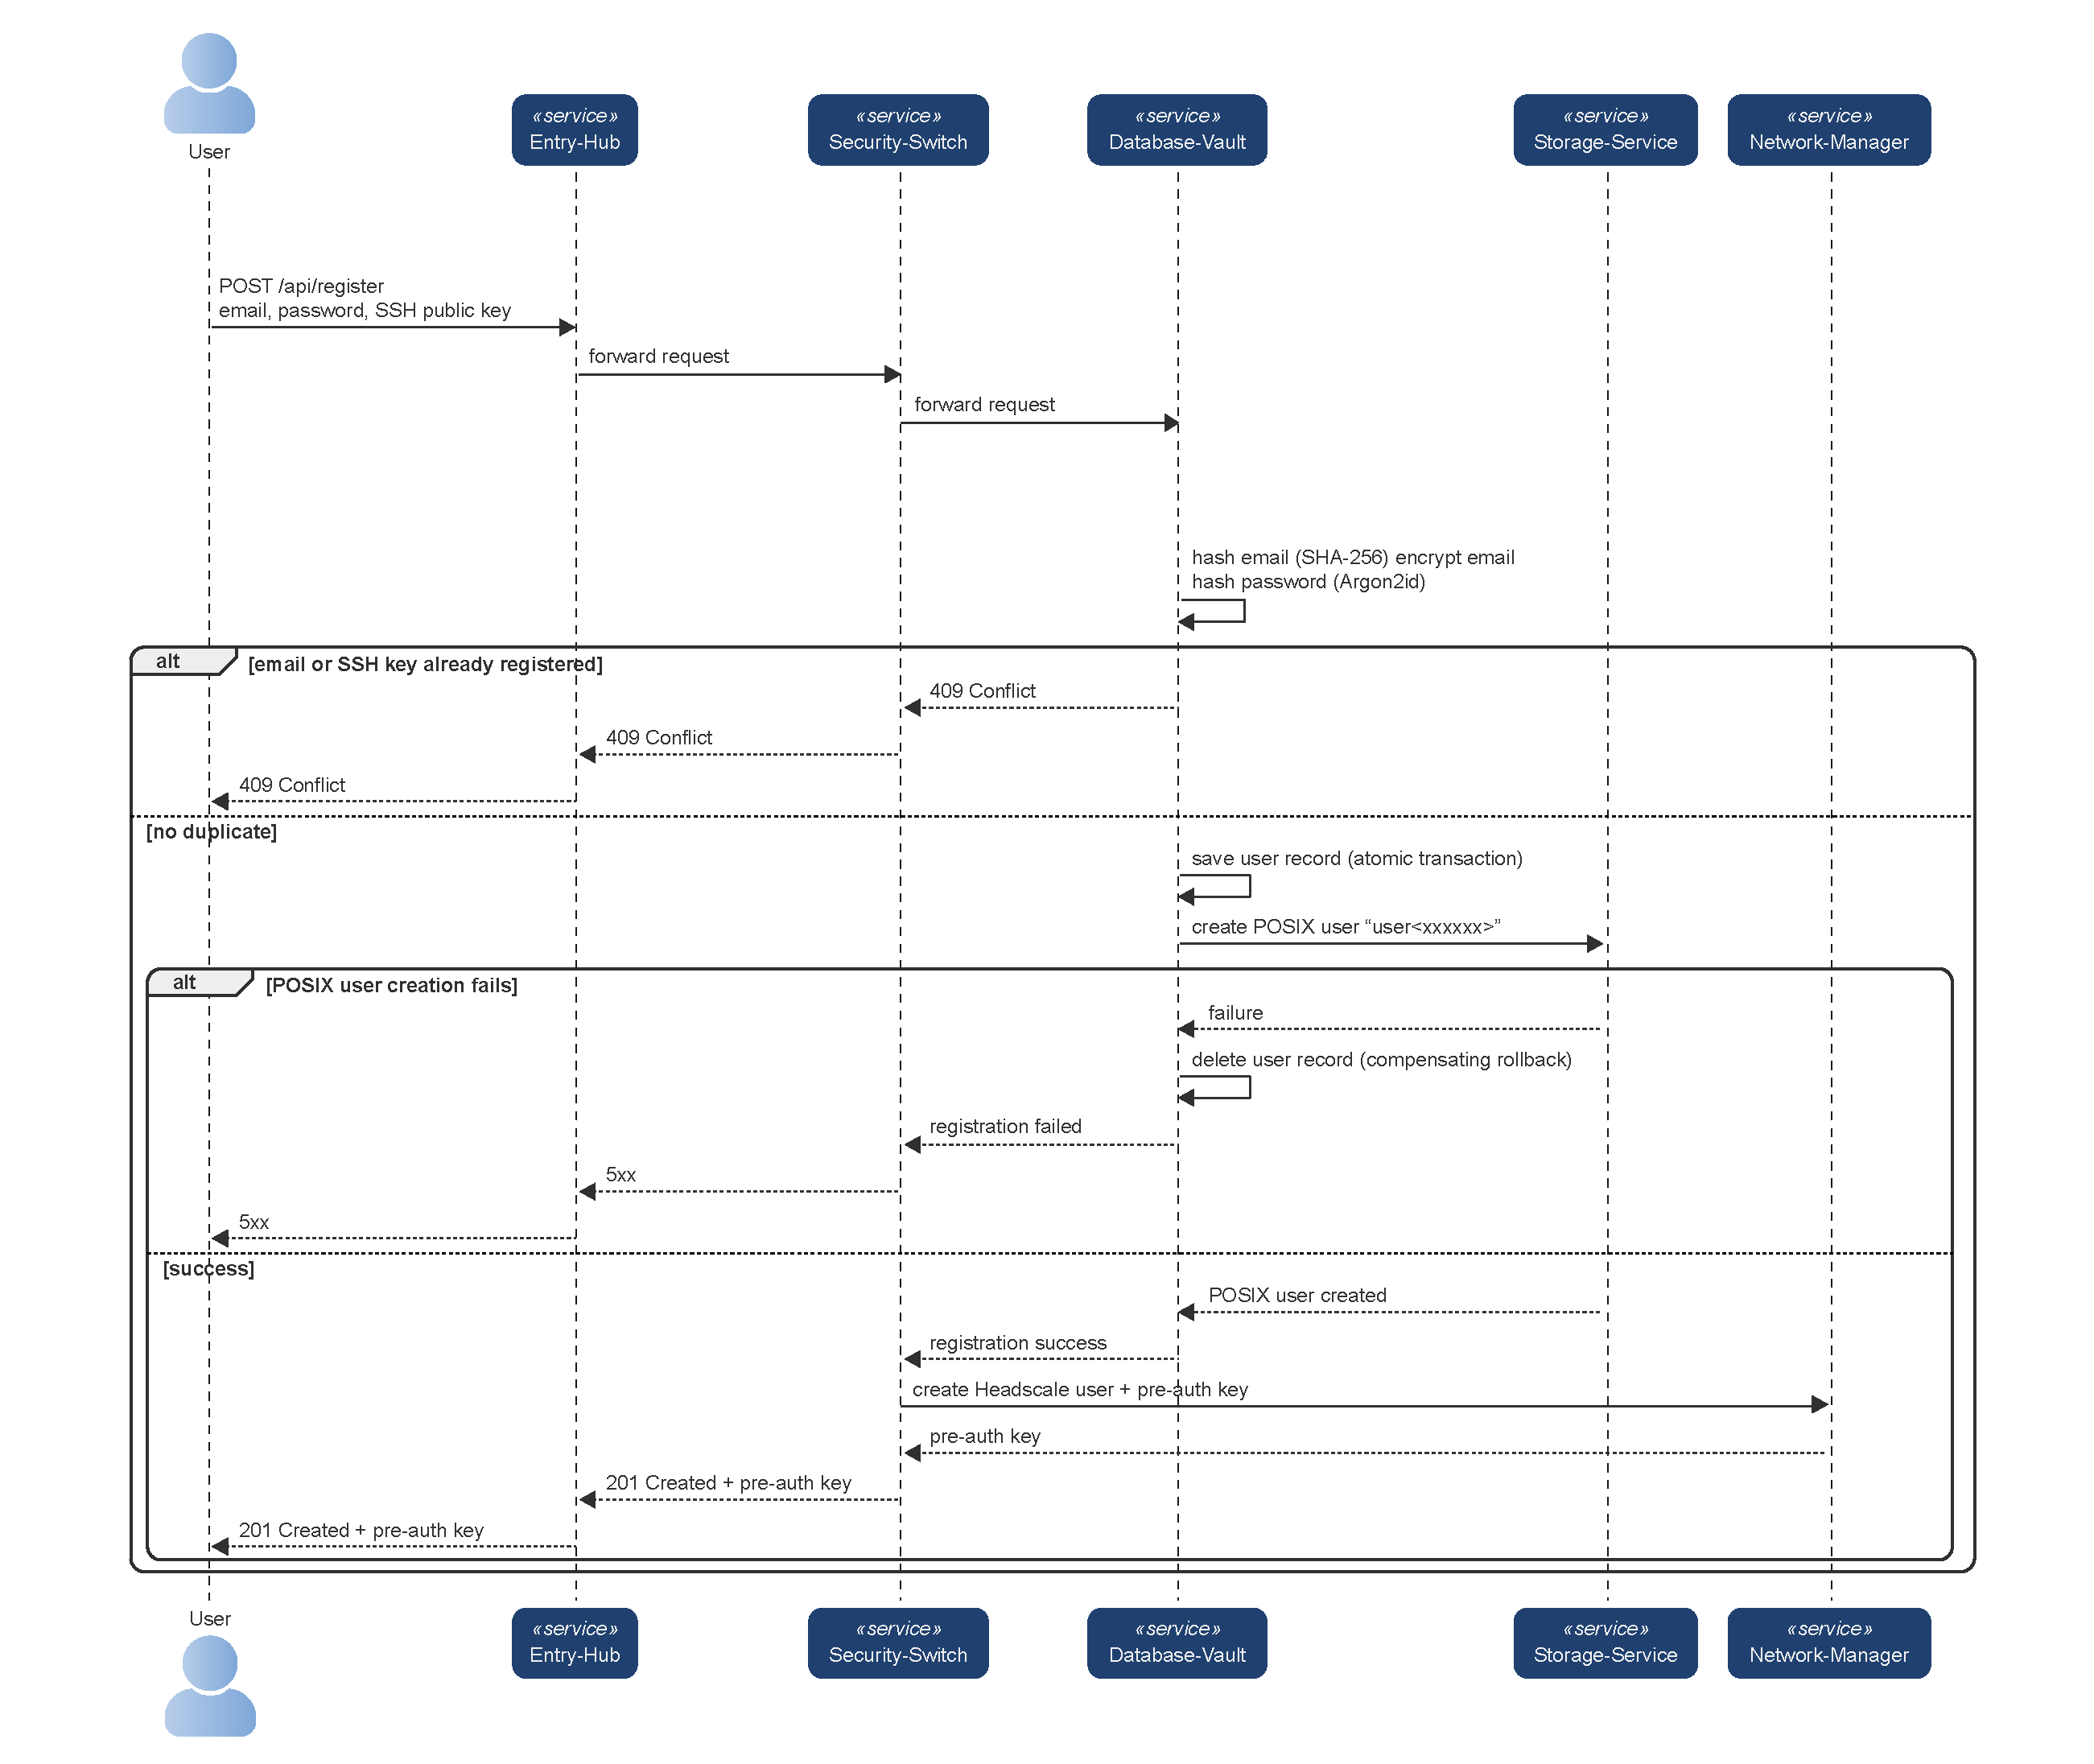
\includegraphics[width=\textwidth]{figures/03-usecases-sequence-uc01-registration.pdf}
    \caption{Registration sequence (UC-01).}
    \label{fig:uc01}
\end{figure}

\section{Login}
\label{sec:login}

During login, Database-Vault recomputes the SHA-256 digest of the received email and uses it to look up the
record.

Salt and cost parameters are extracted from the record's PHC string. Argon2id is recomputed with
those values and with the pepper, and the resulting digest is compared with the stored one through a
constant-time comparison, which therefore does not allow one to infer how many leading bytes of the two values match.

A nonexistent email and a wrong password must produce the same response, and must not
be distinguishable even in the logs. The two paths therefore converge on a single sentinel
error, and the content of the original error is discarded \cite{ramusb-code-login}.

Making the response and the log identical, however, is not enough to make the two cases indistinguishable, because
a third observable difference remains: time. Argon2id, with the parameters of the previous
section, costs tens of milliseconds, and if it were executed only when a record actually
exists, an attacker could distinguish the two situations by measuring the response latency.
The solution adopted is to spend the same time even when there is nothing to verify.

\Needspace{6\baselineskip}
\begin{lstlisting}[caption={Dummy verification used on the rejection paths, from \texttt{hash.go}
\cite{ramusb-code-verify-dummy}.}, label={lst:verifydummy}]
func VerifyDummy(password, pepper []byte) {
	_, _ = VerifyPassword(password, pepper, dummyHash())
}
\end{lstlisting}

The function recomputes Argon2id against a dummy hash, built only once per process with
the same cost parameters as the real records, and discards the result. It is called on every
rejection path, including the one in which the lookup itself fails, so that not even an infrastructure
failure becomes easily measurable from the outside.

Every uncertainty leads to the same outcome. If the verification cannot complete, for example because
the stored hash is malformed, the response remains 401, according to the
fail-secure principle \cite{owasp-fail-securely}. In the logs that case remains distinguishable, because an operator
needs to know whether it is a corrupted record, a careless user, or a genuine attack.

\autoref{fig:uc02} summarizes the complete login sequence, including the branch in which the two causes
of rejection converge on the same response.

\begin{figure}[h]
    \centering
    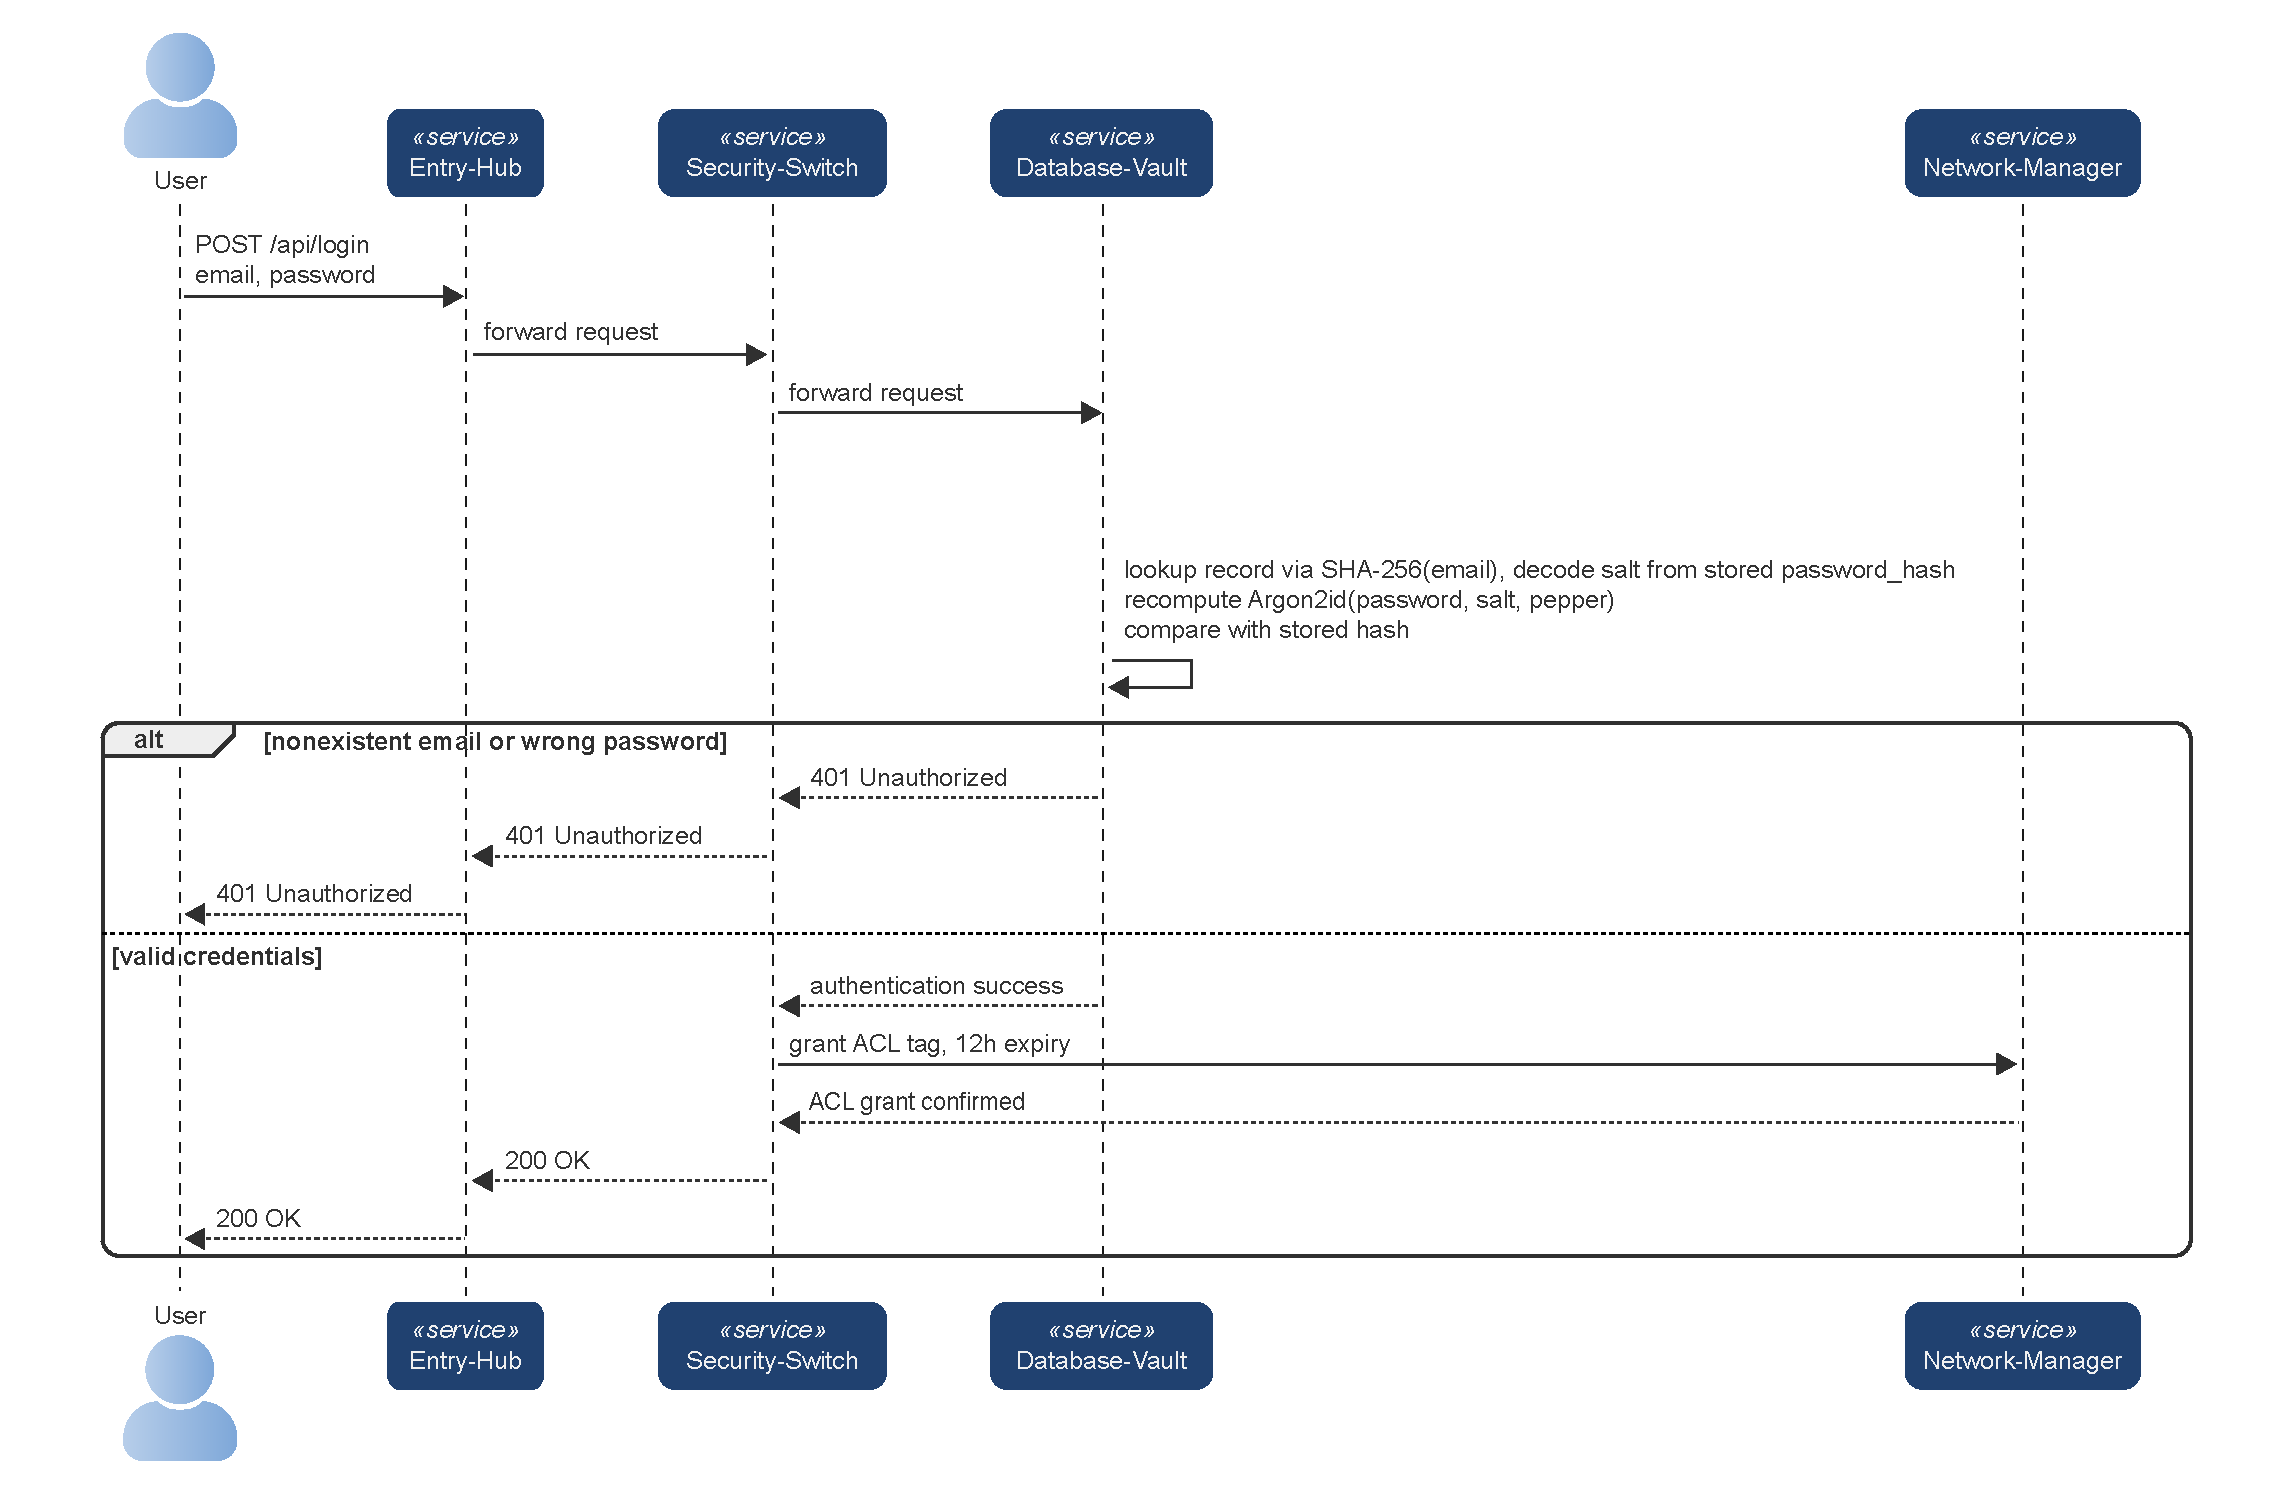
\includegraphics[width=\textwidth]{figures/04-usecases-sequence-uc02-login.pdf}
    \caption{Authentication sequence (UC-02).}
    \label{fig:uc02}
\end{figure}

\section{Post-authentication orchestration}

Authenticating a user, however, still does not give them access to anything. Access, in this system, is
a property of the network. Security-Switch asks Network-Manager to modify the network rules
at two different moments.

After a successful registration, it requests the creation of the user's identity on the mesh network and of
a pre-auth key, which travels back up the chain to the client inside the 201 response and which allows the user's
device to join the private network.

After a successful login, instead, it requests twelve-hour temporary access to Storage-Service.

Both steps, however, grant reachability, not read access: registration puts the
device in the network, login allows it to reach Storage-Service, but what opens the backups is
the SSH private key, which never leaves the user's device.
Knowing the user's credentials is therefore not a sufficient condition to access their backups.

How Network-Manager creates the mesh identity, applies the ACL tag and manages its expiry is the subject
of \autoref{chap:rete}.
